% \documentclass{ijsra}
\def\IJSRAidentifier{\currfilebase} %<---- don’t change this!
\def\submission{}%YYYY-MM-DD
\def\acceptance{}%YYYY-MM-DD
%-------Title | Email | Keywords | Abstract-------------
\def\shorttitle{The Duke of Stone}
\def\maintitle{The Duke of Stone:\\  A new interpretation of Grand Duke Francesco \mbox{de’Medici’s} Renaissance art of politics, \\ explained by Panofsky’s model of iconographical analysis of the Apennine Colossus statue (1580)}
\def\cmail{anneschuitema@gmail.com}
\def\keywords{Renaissance, Tuscany, de’ Medici, Materiality, Symbolism, Panofsky, Statue, Apennine.}
%\def\keywordname{}%<--- redefine the name “Keywords“ in needed language

\def\abstract{This paper offers a new interpretation on the Apennine Colossus statue, accomplished by the Renaissance artist Giambologna and commissioned by the Grand Duke of Tuscany, Francesco I de’Medici (1541–1587). By an overall common iconographic program of a de’ Medici elite, a unique embodiment of a celebrated divinity from antiquity is portrayed which previous researches such as D’Elia (2011), Lazzaro (2011) and Sparitis (2013) did not recognize. However, the layered and subtitle power of the \textit{Colossus} beholds a \textit{heavy intrinsic} meaning that even goes beyond that. This case study questions how power and rulership was legitimized through materiality and symbolism of statues in Renaissance Italy by means of a Panofsky (1955) inspired analysis applied on the \textit{Apennine Colossus} which stand on the foot of a water basin, in the shadows of the Apennine mountain range till this day.}
%--------Author’s names------------
\def\authorone{Anne Schuitema}
%-------Biographical information-------------
\def\bioone{Anne Schuitema is a MA student in Prehistory of Europe and Museum Studies at the
	Faculty of Archaeology, University of Leiden.  When writing this piece, she was a BA student.}
%------University/Institution--------------
\def\affilone{University of Leiden (The Netherlands)}

\begin{filecontents}{\IJSRAidentifier.bib}

@Article{Arba2012,
  author       = {Arba, F. and Inzitari, D. and Barnett, H. J. M. and Lippi, D.},
  title        = {Stroke in Renaissance Time: The Case of Francesco I de’Medici},
  journaltitle = {Cerebrovasc Dis},
  volume       = {33},
  pages        = {589--593},
  date         = {2012},
}

@Book{Burke1989,
  author    = {Burke, P.},
  title     = {Renaissance: History of Europe 1400-1599},
  publisher = {Uitgeverij SUN},
  location  = {Nijmegen (NL)},
  date      = {1989},
}

@Article{DElia2011,
  author       = {D'Elia, U. R.},
  title        = {Giambolognaś Giant and the Cinquecento Villa Garden as a Landscape of Suffering},
  journaltitle = {Studies in the History of Gardens \& Designed Landscapes},
  volume       = {31},
  number       = {3},
  pages        = {1--25},
  date         = {2011},
}

@Book{Dhanens1956,
  author    = {Dhanens, E.},
  title     = {Jean Boulogne: Giovanni Bologna Fiammingo},
  publisher = {Palais Der Academiën},
  location  = {Brussel},
  date      = {1956},
}

@Book{Goudriaan2015,
  author    = {Goudriaan, E. J.},
  title     = {The Cultural Importance of Florentine Patricians: Cultural exchange, brokerage networks, and social representation in Early modern Florence and Rome (1600-1660)},
  publisher = {Optima Grafische Communicatie},
  location  = {Leiden (NL)},
  date      = {2015},
}

@Book{Giannetto2008,
  author    = {Giannetto, R. F.},
  title     = {Medici Gardens from Making to Design},
  publisher = {University of Pennsylvania Press},
  location  = {Pennsylvania (US)},
  date      = {2008},
}

@Book{Goldthwaite2009,
  author    = {Goldthwaite, R. A.},
  title     = {The Economy of Renaissance Florence},
  publisher = {The Johns Hopkins University Press},
  location  = {Baltimore (US)},
  date      = {2009},
}

@Book{Hall1998,
  author    = {Hall, A.},
  title     = {Giambologna},
  publisher = {Salander-O'Reilly Galleries LLC},
  location  = {New York (US)},
  date      = {1998},
}

@Article{Hamburgh1996,
  author       = {Hamburgh, H.},
  title        = {Naldiniś Allegory of Dreams in the Studiolo of Francesco de ́Medici},
  journaltitle = {The Sixteenth Century Journal},
  volume       = {27},
  number       = {3},
  pages        = {679--709},
  date         = {1996},
}

@Book{Hibbert1979,
  author    = {Hibbert, C.},
  title     = {The Rise and Fall of the House of Medici},
  publisher = {Penguin Books Ltd.},
  location  = {London (UK)},
  date      = {1979},
}

@Article{Lazzaro2011,
  author       = {Lazzaro, C.},
  title        = {River Gods: Personifying Nature in Sixteenth-Century Italy},
  journaltitle = {Renaissance Studies},
  volume       = {25},
  number       = {1},
  pages        = {70--94},
  date         = {2011},
}

@Article{Sparitis2013,
  author       = {Sparitis, O.},
  title        = {Sculpture and Environmental Design in the Cultural Landschape of the European countries and Latvia},
  journaltitle = {Landscape Architecture and Art},
  volume       = {2},
  number       = {2},
  pages        = {30--40},
  date         = {2013},
}

@Book{Meskell2009,
  author    = {Meskell, L.},
  title     = {Cosmopolitan Archaeologies},
  publisher = {Duke University Press},
  location  = {London (UK)},
  date      = {2009},
}

@Book{Moormann2007,
  author    = {Moorman, E. M. and Uitterhoeve, W.},
  title     = {Van Alexander tot Zeus: Figuren uit de Klassieke Mythologie en Geschiedenis, met hun Voortleven na de Oudheid},
  publisher = {Uitgeverij SUN},
  location  = {Amsterdam (NL)},
  date      = {2007},
}

@Book{Najemy2006,
  author    = {Najemi, J. M.},
  title     = {A History of Florence},
  publisher = {Blackwell Publishing},
  location  = {Oxford (UK)},
  date      = {2006},
}

@Article{Panofsky1955,
  author       = {Panofsky, E.},
  title        = {Iconography and Iconology: An Introduction to the Study of Renaissance Art},
  journaltitle = {Meaning in the Visual Arts: Papers in and on Art History},
  pages        = {26--54},
  date         = {1955},
}

@Book{Panofsky1963,
  author    = {Panofsky, E.},
  title     = {Studies in Iconology: Humanistic Themes in Renaissance Art},
  publisher = {Harper Torchbooks},
  location  = {New York (US)},
  date      = {1963},
}

@Book{Partridge2009,
  author    = {Partridge, L.},
  title     = {Art of Renaissance Florence 1400-1600},
  publisher = {University of California Press},
  location  = {California (US)},
  date      = {2009},
}

@Incollection{Petersen2011,
  author    = {Petersen, N. H.},
  title     = {Introduction},
  editor    = {Bücker, A. and Ostrem, E. and Petersen, N. H.},
  booktitle = {Resonances: Historical Essays on Continuity and Change},
  publisher = {Brepols Publishers},
  location  = {Turnhout (B)},
  date      = {2011},
}

@Article{Smith1961,
  author       = {Smith, W.},
  title        = {Pratolino},
  journaltitle = {Journal of the Society of Architectural Historians},
  volume       = {20(4)},
  pages        = {155--168},
  date         = {1961},
}

@Incollection{Tanzini2012,
  author    = {Tanzini, L.},
  title     = {Tuscan States: Florence and Siena},
  editor    = {Gamberini, A. and Laccarini, I.},
  booktitle = {The Italian Renaissance},
  publisher = {Cambridge University Press},
  location  = {Cambridge (UK)},
  date      = {2012},
}

@Book{Walsh2015,
  author    = {Walsh, C.},
  title     = {Renaissance Landscapes and he Figuration of Giambolognaś Appennino: An Ecocritical Analysis},
  publisher = {Boston University (PhD)},
  location  = {Boston (US)},
  date      = {2015},
}
\end{filecontents}
\IJSRAopening%<---- don’t change this!
%-------
\IJSRAsection{Introduction}

\lettrine{F}{rom} the fourteenth century onwards, the Medici family built their political power in Florence and Tuscany on their enormous wealth \parencites[93,97]{Tanzini2012}. The de’ Medici family spent enormous amounts of money to strengthen their political ambitions in central Italy, notably through sponsoring the arts and representing themselves as the art’s proverbial protectors. Particularly since the days of Lorenzo il Magnifico (1449-1492), de’ Medici displayed their power, splendour, and grandeur to both their subjects and rivals through countless paintings, books, palace architecture, and statues \cites[685]{Hamburgh1996}[90-91]{Hibbert1979}. In general, (art) historians are well aware the Renaissance elites used a wide variety of art forms to enhance their social and political position \parencites[1]{DElia2011}. However, concerning the de’ Medici family, scholars have primarily been preoccupied with the period when the family rose to great power in the fifteenth to mid-sixteenth centuries. Far less scholarly attention has been given to Grand duke Francesco I de’ Medici (1541-1587), a more obscure and secluded ruler but an equally great interest in the visual arts and the natural sciences \parencites[1-3]{DElia2011}. One great work of art commissioned by Grand duke Francesco may serve as an example of his understanding of visual art to convey a
multi-layered set of political meaning: the huge statue in the gardens of the Pratolino Villa known as \textit{The Colossus of the Apennines} (\cref{fig:Fig1,fig:Fig2,fig:Fig3,fig:Fig4,fig:Fig5,fig:Fig6,fig:Fig7}).\footnote{Today the Villa Medici della Pratolino (constructed between 1569 and 1581) is known as the Villa Demidoff. By the end of the Sixteenth Century there were at least 15 other major Medici estates within a 10 km range of Florence and yet another 11 minor complexes (excl. hunting cottages) in other parts of Tuscany.}

%fig.1
 \begin{figure}[!htb]
	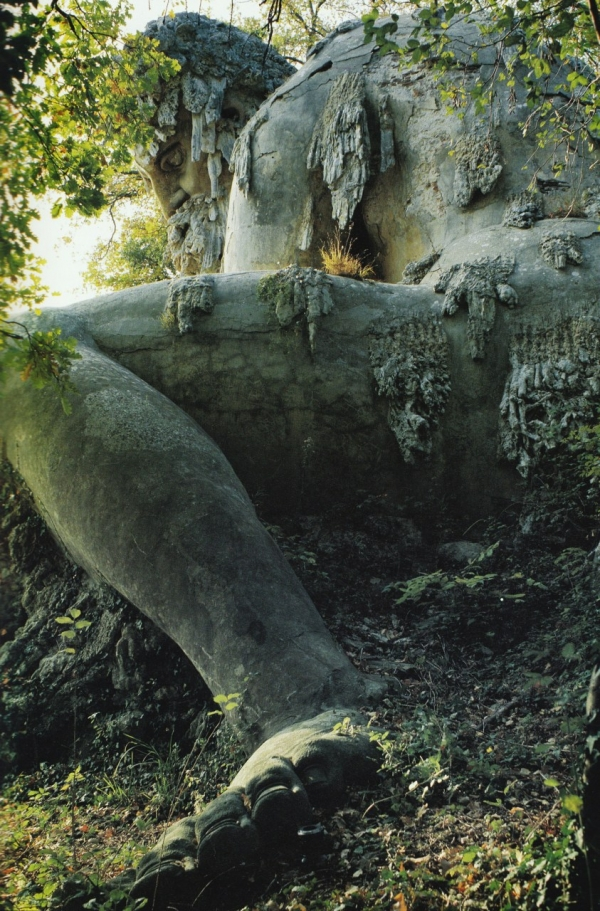
\includegraphics[width=\linewidth]{Schuitema_Fig1}
	\centering
	\caption{A close up from the side of the Appennine Colossus statue (1580) by Giambologna.
		{\normalfont\scriptsize \\ \copyright\ by Anne Schuitema}
		%\shortauthor
		% or NAME OF COPYRIGHT HOLDER
	}
	\label{fig:Fig1}
\end{figure}

The \textit{Colossus} was created by the famous Flemish sculptor Giambologna\footnote{Giambologna was born in Flanders as Jean de Boulogne.}  between 1578 and 1580, and is one of the last great works in the Mannerism style (circa 1520-1580) \parencites[68]{Burke1989}.

The \textit{Apennine Colossus} remains in place since its creation in the gardens of Villa Medici del Pratolino in Vaglia near Florence, Tuscany (Italy) (\cref{fig:Fig8}). The commission by Francesco I de’ Medici, whose motives to create the complex, including the statue, is considered to be of greatest value \parencites[16]{Walsh2015}.\footnote{The complex is now a UNESCO World Heritage site.} Francesco and his father Cosimo I chose the architect Bernardo Buontalenti\footnote{Francesco's "director of spettacoli"}  to design the garden. Unfortunately, most parts of the statue’s archaeological context have been demolished and the rockwork niche once surrounding the statue is no more. Even so, the conspicuous juxtapositions of art and crude nature still ‘stand’ and the complicated iconography of the entirety is embodied in the \textit{Colossus} is subject to a wide range of interpretations.

This paper will critically explore the relationship between this piece of material culture and its commissioner Francesco I, and question how power and rulership were legitimized through materiality and symbolism in late-Renaissance Italy. Through this relationship, a new and deepening allegory of the local Tuscan elite and a nearly forgotten sculpture shall be effectuated \parencites[164]{Meskell2009}. This will be done by applying Panofsky’s model of iconographical analysis to the social-political context of the \textit{Colossus}. Previous scholars have identified the statue as a river god, God himself, the personification of nature in general, the Apennine mountain range itself or do not mention a certain representation at all \parencites[7]{DElia2011}[31]{Sparitis2013}[70]{Lazzaro2011}. Additionally, the statue has not been analysed to its full potential. There is more to it. Through Panofsky’s model, this paper argues that the \textit{Colossus of the Apennines} is both a new, unprecedented representation of a specific and well-known ancient divinity within the sixteenth-century iconographical traditions, and in fact a representation of Francesco himself.

Understanding the intrinsic meaning of the statue - why it is build, its value and power, what it symbolizes and represents - within the full context of sixteenth century iconography involves asking many questions in various scholarly disciplines \parencites[16]{Panofsky1963}. To understand this statue is to understand the contemporary state of philosophy, the political and religious current affairs as well as the iconographic traditions and perhaps the role of the ideological agents of change in the rapidly changing world of (late) Renaissance Italy \parencites[1]{Petersen2011}. By the late 1570’s Grand Duke Francesco was in dire need of legitimization of his rule in the context of increasing external and domestic opposition. The materiality and symbolism of the statue functioned as a propaganda tool to legitimize his power.

Generally speaking, art expresses and represents current changes in society, cultural shifts in thought and world view, and therefore produces different styles and ideals. In short, to understand a work of art is to understand the artist and the (socio-political) context of their time. However, this paper focuses on the client of the artwork rather than the actual artist Giambologna. As will be shown in chapter 3, the \textit{Colossus} statue marks a specific episode in Francesco’s rule. The analysis of this statue will be done by applying Erwin Panofsky’s three-layered model of interpretation to the \textit{Colossus}. These three so-called strata consist of: 1) A bare description of the actual work of art; 2) Connecting artistic motives to greater themes and concepts; 3) Deeper underlying principles, iconological significance and symbolic values \parencites[28-30]{Panofsky1955}.

%fig.2
 \begin{figure}[]
		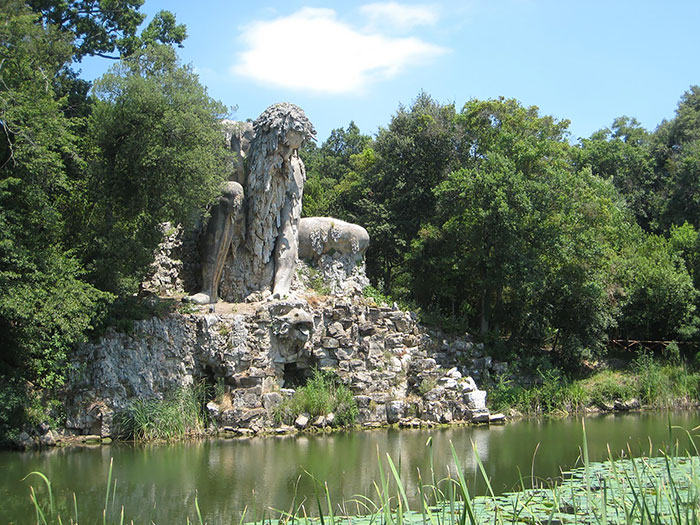
\includegraphics[width=\linewidth]{Schuitema_Fig2}
	\caption{The statue Apennine Colossus (1580) by Giambologna situated in the gardens of Villa Medici at Pratolino, Florence (Italy). \href{https://www.boredpanda.com/appennino-sculpture-colossus-giambologna-florence-italy/}{Source}
		{\normalfont\scriptsize \\ \copyright\ by Andreas Angelidakis
			%\shortauthor
			% or NAME OF COPYRIGHT HOLDER
	}}
		\label{fig:Fig2}

\end{figure}

%fig.3
 \begin{figure}[]
	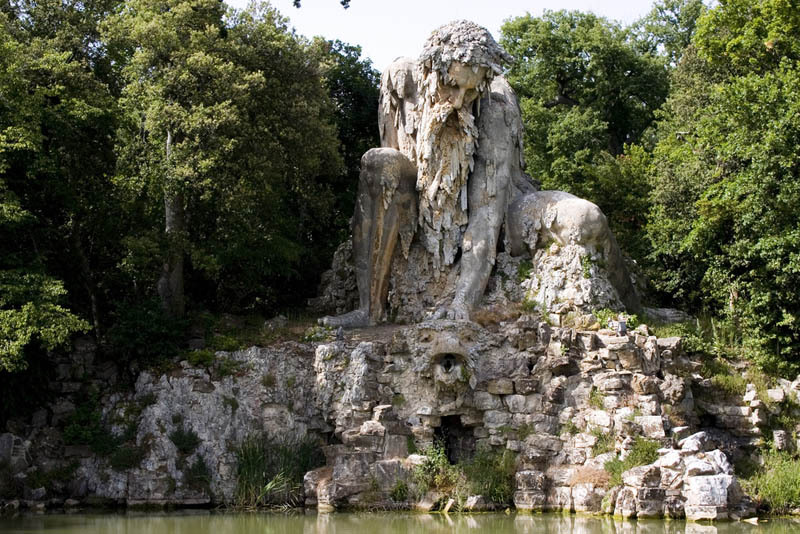
\includegraphics[width=\linewidth]{Schuitema_Fig3}
	\centering
	\caption{A frontal view of the statue Apennine Colossus (1580) by Giambologna. 	\href{https://twistedsifter.com/2012/07/picture-of-the-day-the-statue-of-apennine-by-giambologna/}{Source}
		{\normalfont\scriptsize \\ \copyright\ by  Antonio Scaramuzzino and Anne Schuitema
		%\shortauthor
		% or NAME OF COPYRIGHT HOLDER
	}}
	\label{fig:Fig3}

\end{figure}

%fig.4
\begin{figure}[]
	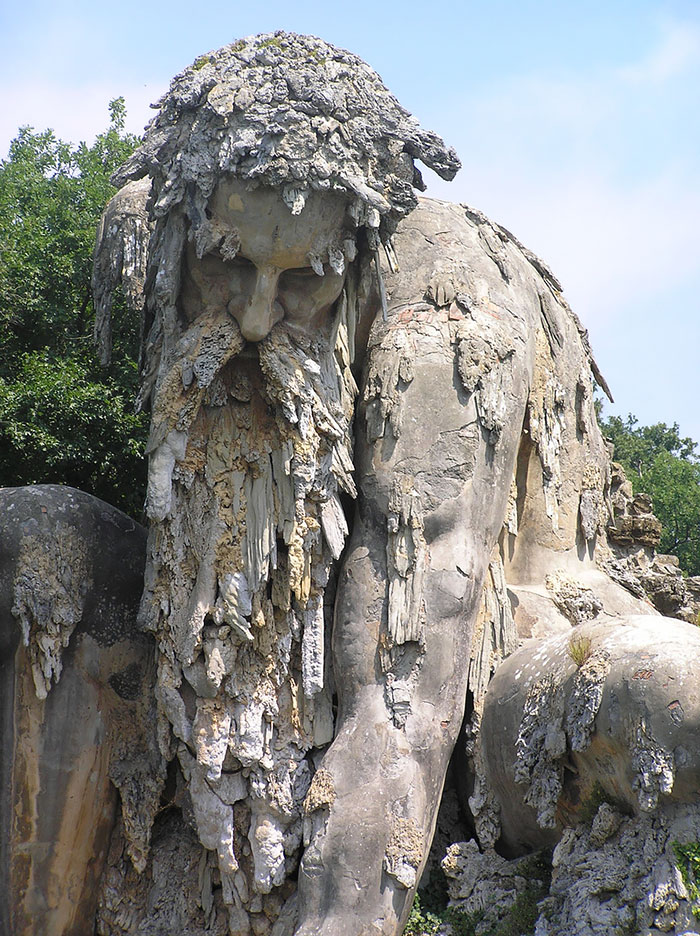
\includegraphics[width=0.7\linewidth]{Schuitema_Fig4}
	\centering
	\caption{A close up of the statue Apennine Colossus (1580) by Giambologna. \href{https://www.boredpanda.com/appennino-sculpture-colossus-giambologna-florence-italy/}{Source}
		{\normalfont\scriptsize \\ \copyright\ by "Delicious Mallicious"
		%\shortauthor
		% or NAME OF COPYRIGHT HOLDER
	}}
	\label{fig:Fig4}

\end{figure}

 %fig.5
 \begin{figure}[]
 	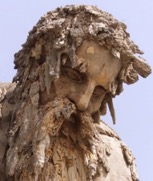
\includegraphics[width=0.7\linewidth]{Schuitema_Fig5}
 	\centering
 	\caption{A close up of the statue Apennine Colossus (1580) by Giambologna. \href{https://mymodernmet.com/giambologna-colosso-dell-appennino/}{Source}
 		{\normalfont\scriptsize \\ \copyright\ by Matteo Bimonte
 		%\shortauthor
 		% or NAME OF COPYRIGHT HOLDER
 	}}
 	\label{fig:Fig5}

 \end{figure}

%fig.6
\begin{figure}[]
	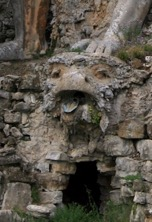
\includegraphics[width=0.7\linewidth]{Schuitema_Fig6}
	\centering
	\caption{Close up of the monster/fountain, a part of the statue Apennine Colossus (1580) by Giambologna. \href{https://mymodernmet.com/giambologna-colosso-dell-appennino/}{Source}
		{\normalfont\scriptsize \\ \copyright\ by Matteo Bimonte
		%\shortauthor
		% or NAME OF COPYRIGHT HOLDER
	}}
	\label{fig:Fig6}

\end{figure}

%fig.7
\begin{figure}[]
	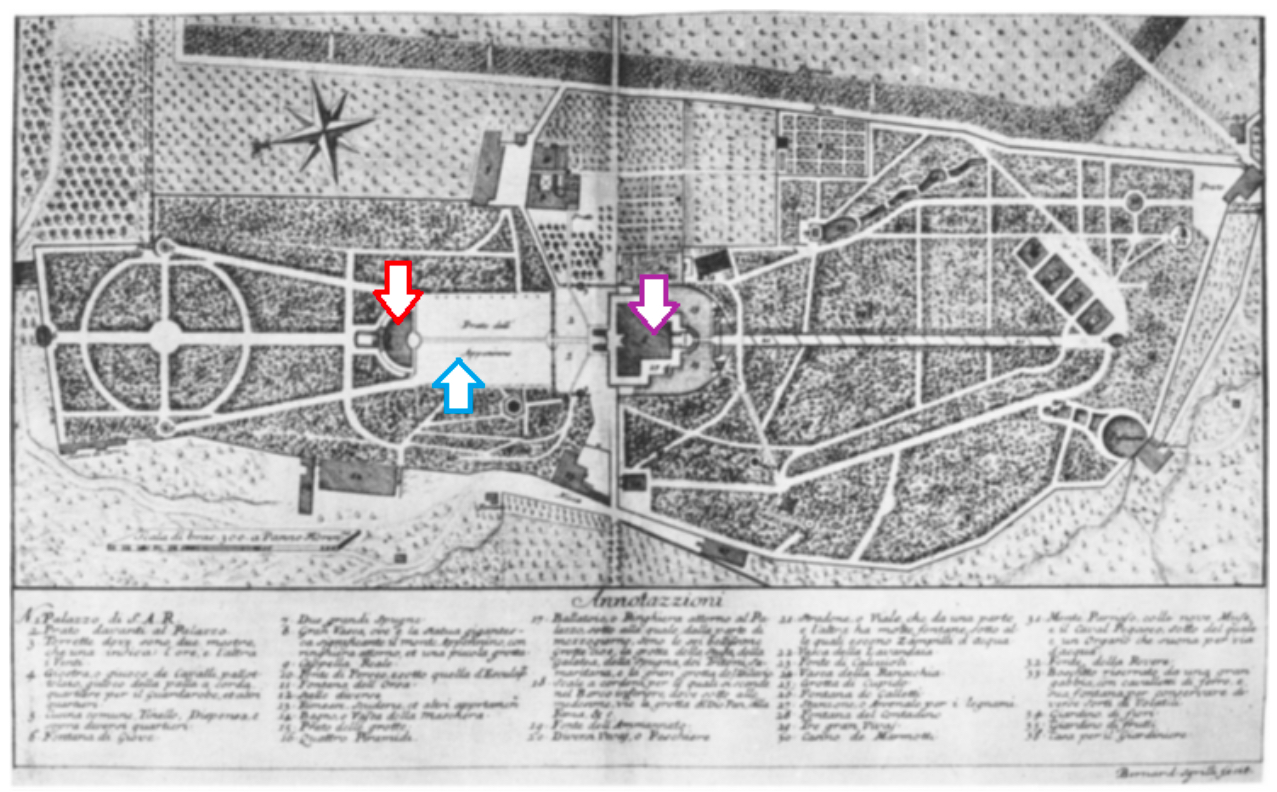
\includegraphics[width=\linewidth]{Schuitema_Fig7}
	\caption{Ground plan of Pratolino’s Villa de’ Medici garden. Map created by Sgrilli in 1742. Arrows: Red= Apennine and pond; Blue= Rectangular clearing Prato dell’Appennino; Purple= the Villa. Source: Smith 1961, 156. (Arrows by author).
		{\normalfont\scriptsize \\ \copyright\ by Anne Schuitema
		%\shortauthor
		% or NAME OF COPYRIGHT HOLDER
	}}
	\label{fig:Fig7}

\end{figure}

%fig.8
\begin{figure}[]
	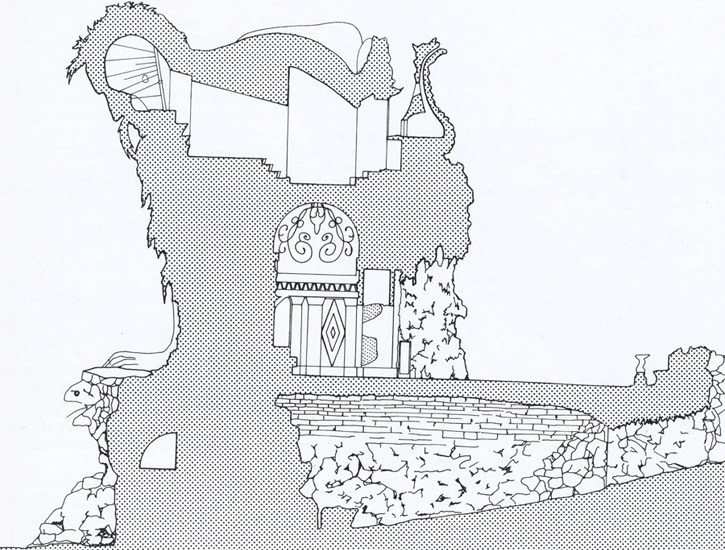
\includegraphics[width=0.9\linewidth]{Schuitema_Fig8}
	\caption{Cross-section of Apennine Colossus (1580) by Giambologna, showing its architectural elements. \href{https://unusualplaces.org/the-appennine-colossus/}{Source}
		\normalfont\scriptsize \\ \copyright\ by P. van der Ree and Anne Schuitema
		%\shortauthor
		% or NAME OF COPYRIGHT HOLDER
	}
	\label{fig:Fig8}

\end{figure}

%fig.9
\begin{figure}[]
	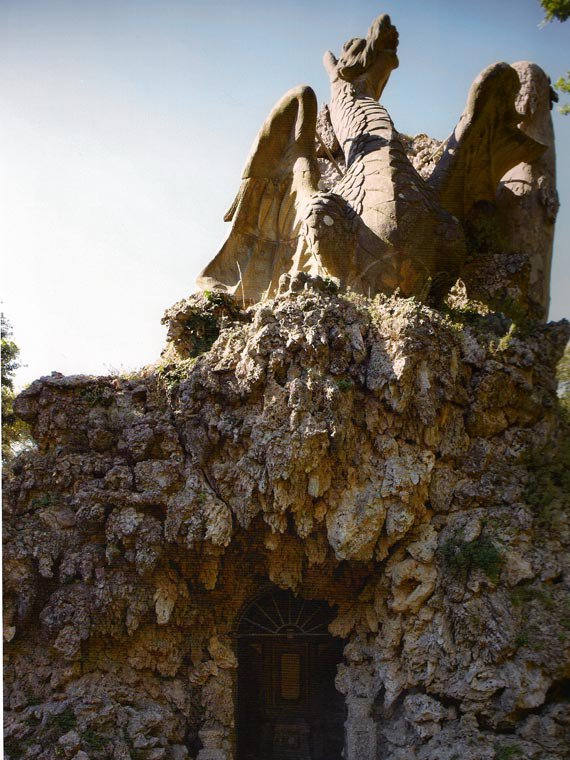
\includegraphics[width=0.7\linewidth]{Schuitema_Fig9}
	\centering
	\caption{The dragon on the back of the Apennine Colossus (1580), above the passage way that leads to the grottoes below and in the sculpture. \href{http://www.grandvoyageitaly.com/piazza/strange-places-in-italy-the-appennine-colossus-a-giant-renaissance-statue-near-florence}{Source}
		{\normalfont\scriptsize \\ \copyright\ by Anne Schuitema
		%\shortauthor
		% or NAME OF COPYRIGHT HOLDER
	}}
	\label{fig:Fig9}

\end{figure}

%fig.10
\begin{figure}[]
	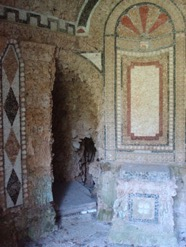
\includegraphics[width=0.7\linewidth]{Schuitema_Fig10}
	\centering
	\caption{The textured walls of mosaic, decorated with collared patterns, sea shells. The dark crack opening in the wall is the entry to a tunnel (south). \href{http://artbyborsheim.blogspot.nl/2010_09_05_archive.html}{Source}.
		{\normalfont\scriptsize \\ \copyright\ by Kelly Borsheim
		%\shortauthor
		% or NAME OF COPYRIGHT HOLDER
	}}
	\label{fig:Fig10}

\end{figure}

%fig.11
\begin{figure}[]
	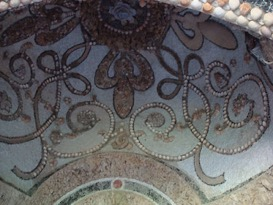
\includegraphics[width=0.7\linewidth]{Schuitema_Fig11}
	\centering
	\caption{A close-up of decoration within the caves and passageways of the Apennine Colossus (1580). \href{http://artbyborsheim.blogspot.nl/2010_09_05_archive.html}{Source}.
		{\normalfont\scriptsize \\ \copyright\ by Kelly Borsheim
		%\shortauthor
		% or NAME OF COPYRIGHT HOLDER
	}}
	\label{fig:Fig11}

\end{figure}


\IJSRAsection{Iconographic layer one – Primary Natural Subject Matter}

As mentioned before, this chapter will provide an identification and enumeration of artistic \textit{motifs} or \textit{pure forms} from the \textit{Apennine Colossus}. This is known as the \textit{pre-iconographical layer} or \textit{primary subject matter} \parencites[28-30]{Panofsky1955}. For practical reasons, this article will not deal with the description and analysis of other parts of the garden unless it directly concerns the statue.

\IJSRAsection{Basic description of the Statue}

The \textit{Apennine Colossus} is an 10.5 meter high statue of a long-bearded man (whose age is difficult to estimate) in a squatting position or as though an extreme \textit{contraposto}. The figure is carved partly out of the mountain\footnote{So the Colossus once was literally part of the Apennine Mountain range.}  that was once surrounding it and is now only framing his bend legs. It consists of tufa, pietra serena sandstone, gypsum and plastered brick and situated within a forest park, posted on a rocky plateau above a turbid pond, almost topping the oaks and cedars around him \parencites[227]{Dhanens1956}[3]{Walsh2015}[2]{DElia2011}.

The giant strikes a controlled reducing pose. The centre of gravity is in the middle and his right arm ‘invisibly’ balancing him fully on a platform behind his bended leg and one bare foot is firmly on the ground. The (small) pose seems not to be weakening his heroic masculine figure. Also, despite its calm yet burdened constitution, it renders strength. The mass of its body is balanced carefully.
His back is hunched, his left shoulder strains lower than the other and exerts down on a circa 1.5 meter large turtle-snake-frog-like head. The perspective chosen by the artist suggests the body of a huge monster that is \textit{de facto} not visible to the spectator because it is one with the rocky underground. This all dramatizes the arduousness of squeezing the water out of the creature’s beak. The man’s own head is bowed and his eyes within his sunken face, are gazing down subdued but vigilant in the direction of the beast. His look is more or less parallel to his left leg, straining lower than his right, leaning this leg and its foot against its rocky base. His torso is compressed in such a fashion that it disappears invisibly behind his crusty, stalactite-like beard.

The alternating natural beige, grey, yellowish colours of the material used, make the margins between the man and the landscape minimal. This is accentuated by the sporadic elongated encrustations of petrified sponge and gypsum dripping from his smooth “fleshy” skin of his shoulders and limbs. Also his haggard and weathered hair is notable.
Even though he shows motion, it looks like he is frozen in time, either emerging from or metamorphosing back into the rough terrain he is made from. Calcified and petrified in time and nature lording with authority.

The statue is located at the north side of the villa garden (\cref{fig:Fig7}). At the back of the statue, not visible to the spectator is a dragon behind the man, above the passageway to the geometric grottoes and inner passageways decorated with mosaic decoration and sea-shells, within and below the man’s massive body (\cref{fig:Fig8,fig:Fig9,fig:Fig10,fig:Fig11}).

The overall rustic appearance of the statue is correlating with the natural environment in general: rhythmical lines, levies and depressions, concave and convex, curves and con-curves, remarkable play of light and shadow. The composition forms a whole and does not feel incomplete. But still the statue looks in some kind of rivalry with its exact location: a once twenty hectare large Villa garden,\footnote{The garden is now circa eighty hectare large.}  miles outside the urban centre, away from other monuments and ruling powers. In the next chapter I will connect these artistic motives to greater themes to eventually reveal the \textit{intrinsic meaning} of the statue.

\IJSRAsection{Iconographic layer two and iconological layer three – Secondary
	Subject Matter and Intrinsic Meaning or Content}

Now that the \textit{motifs} and \textit{composition} of the \textit{Apennine Colossus} are clear, they need to be connected to greater themes and concepts as part of  Panofsky’s second stratum the true iconographical layer. This interpretation will be supported by contextual (historical and archaeological) information. In order to fully grasp the essential, but subjective, meaning “behind” the statue that goes beyond the sphere of conscious volitions, called the \textit{intrinsic meaning}, we need to take a closer look at the socio-political circumstances around the time the statue was built \parencites[6,16]{Panofsky1963}[28-32]{Panofsky1955}.

\IJSRAsection{The socio-political circumstances of Francesco I de’ Medici’s rule}

In 1574, Francesco succeeded his father Cosimo as the second Grand Duke of Tuscany, but had been involved in the domestic policies of the state since the preceding decade. Whereas his father expanded the territorial power of Florence at the expenses of rivals such as Sienna, Ferrera and Modena, Francesco dealt with other Florentine families who had been deprived of their political influence. This new rule by one man was a fundamental break with the past. By 1574, Francesco had established a reputation as a ruthless, cruel prince with no regard for human life. His ascension to the throne was immediately followed by a popular uprising which in turn was put down mercilessly. To complicate matters further, the duchy of Florence played a major part in international politics that forced all Italian princes and city-states to choose one side or the other. Cosimo and Francesco came out of the struggle victoriously and were rewarded by the Pope being elevated from dukes to Grand Dukes. Now, in 1569, they outranked all other Italian rulers but the Pope, intensifying old sores and rivalries. In this context of political and military power struggles we must perceive the \textit{Colossus of the Apennines} in the garden of the Pratolino Villa \parencites[45]{Dhanens1956}[26-33]{Goudriaan2015}[56]{Goldthwaite2009}[250]{Najemy2006}. In 1569, the same year of his elevation to Grand Duke, Cosimo ordered the construction of the garden as a symbol of richness and superior power to his main rival Duke D’Este of Ferrera from whom he had taken away the vacant duchy of Modena. As a well-known Maecenas of the arts he hired one of the best architects available, Buontalenti, in order to impress his rivals \parencites[1]{DElia2011}. The garden itself reflected a common theme in Renaissance culture, namely a representation of the tranquillity, refuge, and harmony of the lost Garden of Eden \parencites[153]{Partridge2009}. In other words, the garden was designed as a symbol of victory as well as a hard-fought, well-earned “peace” \parencites[295-296,302-303]{Goudriaan2015}[168,391]{Goldthwaite2009}.

When Francesco came to power the garden was far from finished, but already filled with art, ponds, waterways and waterworks (jets and fountains), fish tanks, grottoes, cascades, automata and labyrinths, thus being full of surprises. All gave an illusion of a wonder park with living statues and beasts. Despite its given name, the images within the \textit{Apennine} must be interpreted as Herakles, one of the most prominent heroes in classical mythology. Although Herakles is usually identified by his club, which is missing here, he can still be recognized by his damaged cloak of lion skin and the monster he defeated with his bare hands underneath him \parencites[210,216-217]{Moormann2007}. For two main reasons the idea of a huge Herakles statue situated on a mountain was most likely inspired by the life and politics of Grand Duke Francesco himself. Through this statue he compared himself to the great Herakles as a political statement on more than one level \parencites[26,295,303]{Goudriaan2015}[107,168,391,489,513]{Goldthwaite2009}[315,478]{Najemy2006}[216-218]{Moormann2007}.

First, like the Greek prince Herakles, Francesco had to overcome many adversaries (monsters) in order to win his throne.\footnote{According to Greek mythology Herakles was the natural son of Zeus and Alkmene, wife of King Amphitryon of Argos. Herakles was raised as a Prince, but was denied his royal rights by a variety of competitors.}  In one myth Herakles indeed slayed a dragon. He would be tested time and again, but would eventually prevail. In Francesco’s case, his reign in 1574 started with a failed conspiracy to murder the whole Medici family. Besides that,  his claims to the huge parts of Tuscany were contested by rival princes who were defeated one by one. By positioning Herakles on top of the \textit{Apennines}, which is the mountain range that separated Francesco’s territory from his main enemy to the north (Duke D’Este of Ferrera), he proclaimed himself as the leading prince of Central Italy. This statement of ‘height’ here means literally ‘being on top’. Also the statue is facing the north towards D’Este (\cref{fig:Fig7}). Considering the fact that the statue was issued in 1579, it also refers to the crushing of two uprisings against his rule in Florence only a few years before (1575 and 1578). These confrontations remind us of Herakles’ struggle with the Hydra of Lerna, a dragon-like beast whose undead head he buried beneath a rock. He literally squashes the water (life) out of the monster’s beak (\cref{fig:Fig6}). The deeper symbolic level is a political and military analogy of Herakles’ bravery and righteousness by defeating his enemies bare-handedly. These acts of defeating evil and betrayal purified Herakles from his sins \parencites[207-209;211]{Moormann2007}.

Secondly, the statue is closely related to Francesco’s marital life, also of great political importance. Since 1565 he was married to Johanna of Austria, daughter of the Holy Roman Emperor Ferdinand I. This was a typical political marriage of convenience, for his true love was his long-term mistress of lower birth, Bianca Cappello from Venice, for whom he had built the Villa Pratolino in the first place. Within two months after Johanna’s mysterious death in 1578 he married Bianca \parencites[589-90]{Arba2012}. Because Francesco’s subjects frowned upon both his late wife’s death and his new morganatic marriage, the official celebrations of the latter took place a year later in the gardens around the same time Giambologna had started constructing the \textit{Colossus}. Again, there is a close analogy with Herakles’ adventures. In his last battle, the ancient hero was stripped of his lion cloak and club by his secret lover (who had ‘tamed’ him). His jealous wife, who, like Johanna, was the daughter of a monarch, tried to kill him as soon as she learned about the affair. She drained his lion cloak in poisonous blood which caused Herakles great agony. Like a fire-burn he could not remove it without tearing off parts of his skin. A close look at the statue, also reveals bits and pieces of the said cloak\footnote{In the myth Herakles' wife kills herself and he receives a beautiful new replacement. The myth corresponds with Christianity too. His suffering from the poison compared to the suffering of Christ on the Calvary. Negatively, Herakles can act as a pagan image of the Old Testament, with the core-message "an eye for an eye" \parencites[211,213,214-218]{Moormann2007}} (\cref{fig:Fig1} and \cref{fig:Fig4}) \parencites[211-213]{Moormann2007}[XI-XIII]{Hall1998}.

\IJSRAsection{Princes; Mannerism and Humanism}

By posing as Herakles, Francesco made use of a typical Renaissance form of artistic propaganda inspired by antiquity. Rulers often portrayed themselves as Herakles, the symbol of (their) virtues, military might and power. This iconography dominates sixteenth-century visual culture of elite residences, urban centres and regal parks. References to Herakles imply purposefulness, thoroughness, human virtue, heroism (of a perfect knight), a good ruler, faith, and an imbued knowledge of the heavy duties he has to fulfil and therefore deserving \textit{apotheosis}. The imitation of classical arts was the hallmark of western culture in the Renaissance era.\footnote{The assumption that Renaissance Italy was the runner up in activity, creativity and regeneration is incorrect but nevertheless indispensable when talking about this period. In Italy many influences of Greek and Roman mythology were still visually present in many forms of art and architecture.}  The Herakles-iconography stems from the contemporary movement of Humanism. The ancients were honoured in this context because they presented a renewed, superior guide to perfecting humanity. The highly valued appearance of things representing what is “real” or “truly natural” to the artist (Realism) is also shown in sculpt  \parencites[7,13,16,23-24,39,43]{Burke1989}[56]{Goldthwaite2009}[250]{Najemy2006}[211,213-218]{Moormann2007}. With this, the ambiguous Mannerist style highlighted all the mentioned qualities: the dramatic effect by experimenting, ingenuity and bending the “rules” can be well translated back to the \textit{Apennine} statue \parencites[69,71-72]{Burke1989}[396]{Goldthwaite2009}. This mannerist fashion is also present in the Pratolino garden as a whole, with its grottoes, mechanics, irrigation systems, waterworks, mystique touches and some artistic freedom. Gardens like Pratolino were common in sixteenth-century Tuscany. In sculpture, the slender and twisted human form, \textit{figura serpentinat} or \textit{contraposto}, posture was also a clear main feature of Mannerism. Composing figures were also frequently displayed by Giambologna’s other sculptures such as: \textit{Florence triumphant over Pisa} (1564), \textit{Fountain of Neptune} (1563-1566), \textit{Rape of the Sabines} (1579-1582), \textit{Hercules Slaying a Centaur} (1595-1600), \textit{Mercury} (1565)\footnote{The latter he created as a diplomatic gift from the Medici to the Holy Roman Emperor.} \parencites[42-44]{Burke1989}[155,161,163]{Smith1961}[34-36]{Dhanens1956}[200]{Partridge2009}[XI-XII]{Hall1998}.

Cosimo I founded the first (art) Academy of Design in 1563, in order to centralize control over all the arts \parencites[9,200]{Partridge2009}.
The same goes for Francesco%
\footnote{He established a private "museum" and collected (precious) stones. These private rooms where often used to talk to his close "friend" Giambalogna. Undeniably, the personality, creative imagination, excesses, sense/attraction of/to greatness vagaries of Francesco acted on Giambologna and gave impulse to great artistic experiments like the \textit{Apennine}.}  % Lukas inserted a } for closing footnote (line 405)
and his ‘designers’ who understood that  the ancients proved to be very useful to propagandize visually the legitimacy of the Grand Duke’s monarchical power as a (lawful) replacement of the old \textit{Republican} traditions. His self-image as Herakles is a godly allegory that sent a clear (political) message \parencites[295-296,302-303]{Goudriaan2015}[168,391]{Goldthwaite2009}.

\IJSRAsection{Conclusion}

The de’ Medici created status in many ways. One of them was a high cultural, artistic and iconographic program to impress and commit rulers and common folk. They never missed an opportunity to propagate their political messages and their (inter)national position. The \textit{Apennine Colossus} and the Pratolino complex as a whole are good examples of this. Many images carry a secondary subject matter. Not all expressional qualities of the statue correspond with the myth of Herakles or are not even expressed at all by the artist or investigated fully in this piece. Even so, purposely or not, the Maecenas Francesco and the “other” artist Giambologna created a highly meaningful and symbolic piece. By applying Panofsky’s model of iconography to analyse the social-political context of Francesco de’ Medici’s elite ruling and Renaissance Tuscany, levels of meaning within the \textit{Apennine} sculpture have been resented from a different perspective. It shows that the \textit{Colossus of the Apennines} is both a new representation of Herakles within the sixteenth-century iconographical traditions, and in fact a representation of Francesco himself. The relationship between materiality and the creator(s) can tell unique and powerful allegories that should not be underestimated.

As a sequel to this Francesco-centred narrative it is necessary to investigate all the aspects of sixteenth century Florence, the garden with all its statues and innovations and the Villa. This way an even more dynamic message can be sketched with the uncovering of more compelling secrets, forgotten Renaissance lives and choices, and the intertwined lives of the four main characters:\footnote{Thus, Cosimo, Francesco, Giambologna \textit{and} Bountalenti.}  ghosts of the past can be re-lived and stripped of their propagandistic cover to reveal the true personal stories. Like Francesco - a Grand Duke with a heart of stone.



%\IJSRAseparator


\IJSRAclosing%<---- don’t change this!
